%!TEX root = ../template.tex
%%%%%%%%%%%%%%%%%%%%%%%%%%%%%%%%%%%%%%%%%%%%%%%%%%%%%%%%%%%%%%%%%%%%
%% chapter4.tex
%% NOVA thesis document file
%%
%% Chapter with lots of dummy text
%%%%%%%%%%%%%%%%%%%%%%%%%%%%%%%%%%%%%%%%%%%%%%%%%%%%%%%%%%%%%%%%%%%%

\typeout{NT FILE chapter4.tex}%

\chapter{Planning}
\label{cha:Planning}

This chapter outlines the timeline and milestones for the development of the proposed AI-driven tool. The planning process is structured to ensure efficient progress across all stages, from initial data collection and preprocessing to model development, evaluation, and deployment. A detailed Gantt chart is provided to visualize the schedule, ensuring that tasks are completed on time and resources are allocated effectively.
\section{Timeline & Milestones}
The project is divided into several key phases, each with specific deliverables and deadlines. The timeline is designed to accommodate iterative refinement and unforeseen challenges, ensuring a robust and reliable outcome.
\begin{figure}[h]
\centering
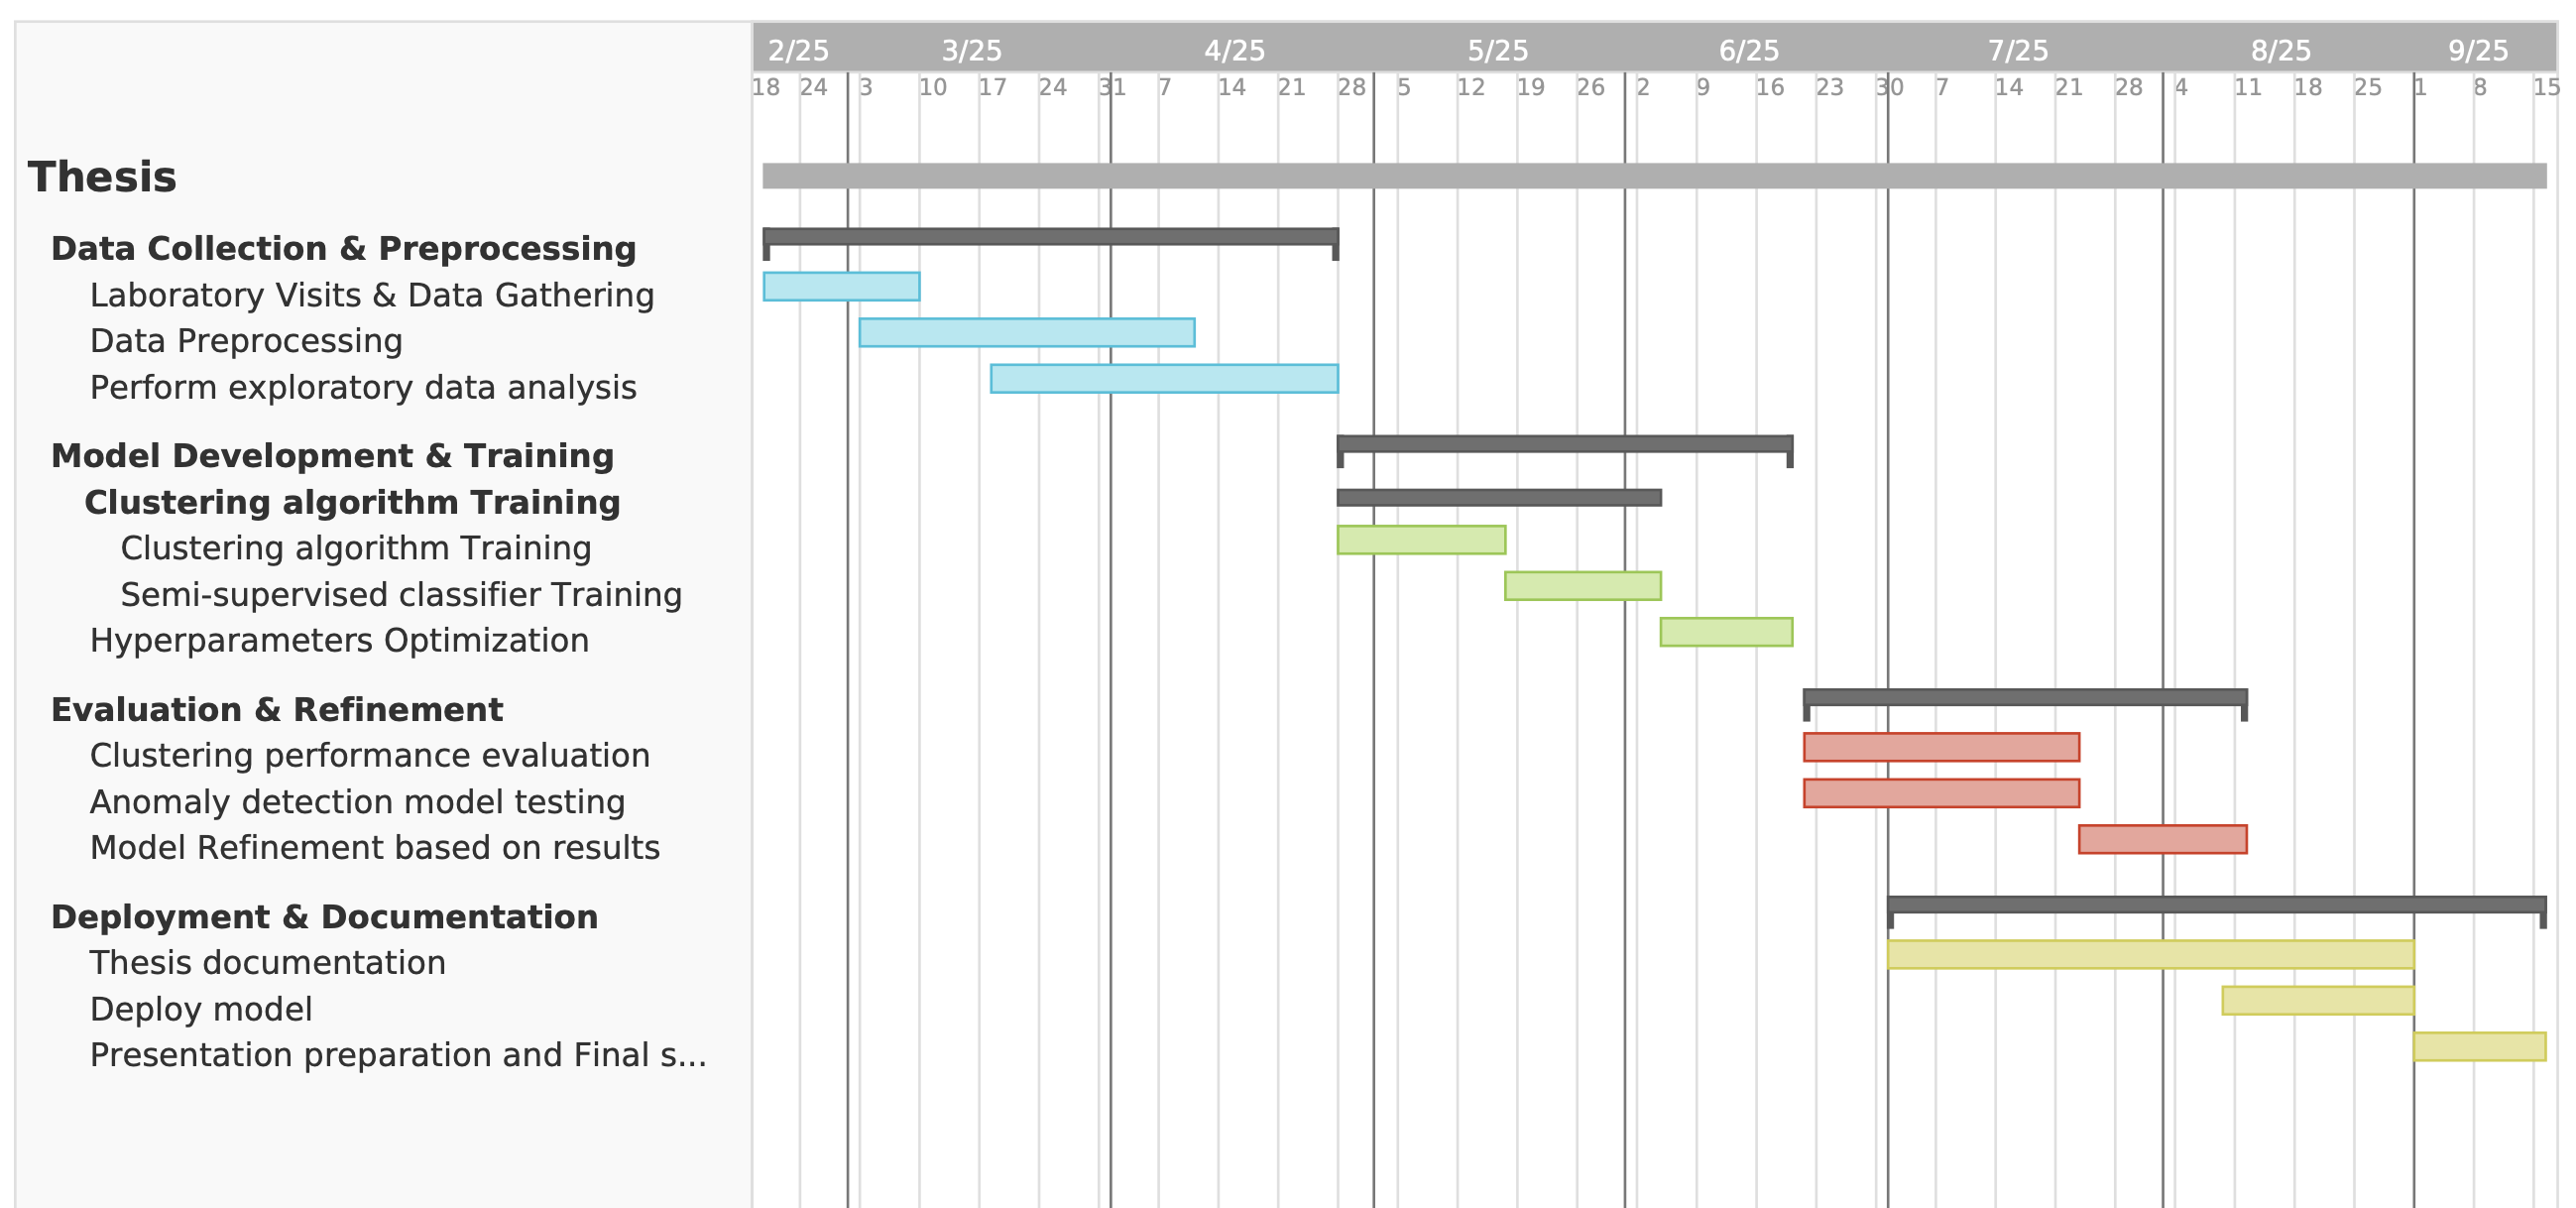
\includegraphics[width=\textwidth]{gantt.png} 
\caption{Gantt Chart of the Project Timeline}
\label{fig:gantt}
\end{figure}
The Gantt chart (Figure \ref{fig:gantt}) illustrates the following phases:
\begin{itemize}
\item \textbf{Phase 1:} Data Collection & Preprocessing (Months 1–2)
\item \textbf{Phase 2:} Model Development & Training (Months 3–5)
\item \textbf{Phase 3:} Evaluation & Refinement (Months 6–7)
\item \textbf{Phase 4:} Deployment & Documentation (Months 8–9)
\end{itemize}